\documentclass[twocolumn]{aastex62}
\usepackage{xspace}

%% The default is a single spaced, 10 point font, single spaced article.
%% There are 5 other style options available via an optional argument. They
%% can be envoked like this:
%%
%% \documentclass[argument]{aastex62}
%% 
%% where the layout options are:
%%
%%  twocolumn   : two text columns, 10 point font, single spaced article.
%%                This is the most compact and represent the final published
%%                derived PDF copy of the accepted manuscript from the publisher
%%  manuscript  : one text column, 12 point font, double spaced article.
%%  preprint    : one text column, 12 point font, single spaced article.  
%%  preprint2   : two text columns, 12 point font, single spaced article.
%%  modern      : a stylish, single text column, 12 point font, article with
%% 		  wider left and right margins. This uses the Daniel
%% 		  Foreman-Mackey and David Hogg design.
%%  RNAAS       : Preferred style for Research Notes which are by design 
%%                lacking an abstract and brief. DO NOT use \begin{abstract}
%%                and \end{abstract} with this style.
%%
%% Note that you can submit to the AAS Journals in any of these 6 styles.
%%
%% There are other optional arguments one can envoke to allow other stylistic
%% actions. The available options are:
%%
%%  astrosymb    : Loads Astrosymb font and define \astrocommands. 
%%  tighten      : Makes baselineskip slightly smaller, only works with 
%%                 the twocolumn substyle.
%%  times        : uses times font instead of the default
%%  linenumbers  : turn on lineno package.
%%  trackchanges : required to see the revision mark up and print its output
%%  longauthor   : Do not use the more compressed footnote style (default) for 
%%                 the author/collaboration/affiliations. Instead print all
%%                 affiliation information after each name. Creates a much
%%                 long author list but may be desirable for short author papers
%%
%% these can be used in any combination, e.g.
%%
%% \documentclass[twocolumn,linenumbers,trackchanges]{aastex62}
%%
%% AASTeX v6.* now includes \hyperref support. While we have built in specific
%% defaults into the classfile you can manually override them with the
%% \hypersetup command. For example,
%%
%%\hypersetup{linkcolor=red,citecolor=green,filecolor=cyan,urlcolor=magenta}
%%
%% will change the color of the internal links to red, the links to the
%% bibliography to green, the file links to cyan, and the external links to
%% magenta. Additional information on \hyperref options can be found here:
%% https://www.tug.org/applications/hyperref/manual.html#x1-40003
%%
%% If you want to create your own macros, you can do so
%% using \newcommand. Your macros should appear before
%% the \begin{document} command.
%%
\newcommand{\vdag}{(v)^\dagger}
\newcommand\aastex{AAS\TeX}
\newcommand\latex{La\TeX}

\newcommand{\Gray}{$\gamma$~ray\xspace}
\newcommand{\Grays}{$\gamma$~rays\xspace}
\newcommand{\GRays}{$\gamma$~Rays\xspace}
\newcommand{\gray}{$\gamma$-ray\xspace}
\newcommand{\unit}[1]{\,\mathrm{#1}\xspace}
\newcommand{\Fermi}{\emph{Fermi}\xspace}
\newcommand{\FermiLAT}{\emph{Fermi}~LAT\xspace}
\newcommand{\fermiLAT}{\emph{Fermi}-LAT\xspace}
\newcommand{\todo}[1]{\textbf{\textcolor{red}{#1}}}

%% Reintroduced the \received and \accepted commands from AASTeX v5.2
\received{\today}
\revised{January 7, 2019}
\accepted{Soon}
%% Command to document which AAS Journal the manuscript was submitted to.
%% Adds "Submitted to " the arguement.
\submitjournal{ApJ}

%% Mark up commands to limit the number of authors on the front page.
%% Note that in AASTeX v6.2 a \collaboration call (see below) counts as
%% an author in this case.
%
%\AuthorCollaborationLimit=3
%
%% Will only show Schwarz, Muench and "the AAS Journals Data Scientist 
%% collaboration" on the front page of this example manuscript.
%%
%% Note that all of the author will be shown in the published article.
%% This feature is meant to be used prior to acceptance to make the
%% front end of a long author article more manageable. Please do not use
%% this functionality for manuscripts with less than 20 authors. Conversely,
%% please do use this when the number of authors exceeds 40.
%%
%% Use \allauthors at the manuscript end to show the full author list.
%% This command should only be used with \AuthorCollaborationLimit is used.

%% The following command can be used to set the latex table counters.  It
%% is needed in this document because it uses a mix of latex tabular and
%% AASTeX deluxetables.  In general it should not be needed.
%\setcounter{table}{1}

%%%%%%%%%%%%%%%%%%%%%%%%%%%%%%%%%%%%%%%%%%%%%%%%%%%%%%%%%%%%%%%%%%%%%%%%%%%%%%%%
%%
%% The following section outlines numerous optional output that
%% can be displayed in the front matter or as running meta-data.
%%
%% If you wish, you may supply running head information, although
%% this information may be modified by the editorial offices.
\shorttitle{Sample article}
\shortauthors{Meyer et al.}
%%
%% You can add a light gray and diagonal water-mark to the first page 
%% with this command:
% \watermark{text}
%% where "text", e.g. DRAFT, is the text to appear.  If the text is 
%% long you can control the water-mark size with:
%  \setwatermarkfontsize{dimension}
%% where dimension is any recognized LaTeX dimension, e.g. pt, in, etc.
%%
%%%%%%%%%%%%%%%%%%%%%%%%%%%%%%%%%%%%%%%%%%%%%%%%%%%%%%%%%%%%%%%%%%%%%%%%%%%%%%%%

%% This is the end of the preamble.  Indicate the beginning of the
%% manuscript itself with \begin{document}.

\begin{document}

\title{Characterizing the brightest gamma-ray flares of flat spectrum radio quasars}

%% LaTeX will automatically break titles if they run longer than
%% one line. However, you may use \\ to force a line break if
%% you desire. In v6.2 you can include a footnote in the title.

%% A significant change from earlier AASTEX versions is in the structure for 
%% calling author and affilations. The change was necessary to implement 
%% autoindexing of affilations which prior was a manual process that could 
%% easily be tedious in large author manuscripts.
%%
%% The \author command is the same as before except it now takes an optional
%% arguement which is the 16 digit ORCID. The syntax is:
%% \author[xxxx-xxxx-xxxx-xxxx]{Author Name}
%%
%% This will hyperlink the author name to the author's ORCID page. Note that
%% during compilation, LaTeX will do some limited checking of the format of
%% the ID to make sure it is valid.
%%
%% Use \affiliation for affiliation information. The old \affil is now aliased
%% to \affiliation. AASTeX v6.2 will automatically index these in the header.
%% When a duplicate is found its index will be the same as its previous entry.
%%
%% Note that \altaffilmark and \altaffiltext have been removed and thus 
%% can not be used to document secondary affiliations. If they are used latex
%% will issue a specific error message and quit. Please use multiple 
%% \affiliation calls for to document more than one affiliation.
%%
%% The new \altaffiliation can be used to indicate some secondary information
%% such as fellowships. This command produces a non-numeric footnote that is
%% set away from the numeric \affiliation footnotes.  NOTE that if an
%% \altaffiliation command is used it must come BEFORE the \affiliation call,
%% right after the \author command, in order to place the footnotes in
%% the proper location.
%%
%% Use \email to set provide email addresses. Each \email will appear on its
%% own line so you can put multiple email address in one \email call. A new
%% \correspondingauthor command is available in V6.2 to identify the
%% corresponding author of the manuscript. It is the author's responsibility
%% to make sure this name is also in the author list.
%%
%% While authors can be grouped inside the same \author and \affiliation
%% commands it is better to have a single author for each. This allows for
%% one to exploit all the new benefits and should make book-keeping easier.
%%
%% If done correctly the peer review system will be able to
%% automatically put the author and affiliation information from the manuscript
%% and save the corresponding author the trouble of entering it by hand.

\correspondingauthor{Manuel Meyer}
\email{mameyer@stanford.edu}

\author[0000-0002-0738-7581]{Manuel Meyer}
\affil{Kavli}

\author{The \emph{Fermi}-LAT Collaboration}
\affiliation{Flying from a low Earth orbit}

%% Note that the \and command from previous versions of AASTeX is now
%% depreciated in this version as it is no longer necessary. AASTeX 
%% automatically takes care of all commas and "and"s between authors names.

%% AASTeX 6.2 has the new \collaboration and \nocollaboration commands to
%% provide the collaboration status of a group of authors. These commands 
%% can be used either before or after the list of corresponding authors. The
%% argument for \collaboration is the collaboration identifier. Authors are
%% encouraged to surround collaboration identifiers with ()s. The 
%% \nocollaboration command takes no argument and exists to indicate that
%% the nearby authors are not part of surrounding collaborations.

%% Mark off the abstract in the ``abstract'' environment. 
\begin{abstract}

Abstract

\end{abstract}

%% Keywords should appear after the \end{abstract} command. 
%% See the online documentation for the full list of available subject
%% keywords and the rules for their use.
\keywords{editorials, notices --- 
miscellaneous --- catalogs --- surveys}

%% From the front matter, we move on to the body of the paper.
%% Sections are demarcated by \section and \subsection, respectively.
%% Observe the use of the LaTeX \label
%% command after the \subsection to give a symbolic KEY to the
%% subsection for cross-referencing in a \ref command.
%% You can use LaTeX's \ref and \label commands to keep track of
%% cross-references to sections, equations, tables, and figures.
%% That way, if you change the order of any elements, LaTeX will
%% automatically renumber them.
%%
%% We recommend that authors also use the natbib \citep
%% and \citet commands to identify citations.  The citations are
%% tied to the reference list via symbolic KEYs. The KEY corresponds
%% to the KEY in the \bibitem in the reference list below. 

\section{Introduction} \label{sec:intro}

More than half of the sources observed with the \Fermi Large Area Telescope (LAT) above 100 MeV are active galaxies that produce particle outflows (jets) at almost the speed of light, which are closely aligned to the line of sight.\footnote{See e.g. \url{http://www.asdc.asi.it/fermi3fgl/}}
%Yet, the exact mechanism and location of \gray production inside such jets of these so-called blazars remain a controversially discussed topic in the literature~\cite{Madejski:2016oqg}.
The broadband electromagnetic radiation observed from these so-called blazars spans decades in energy from radio frequencies up to very-high energy \gray energies. 
It is often described with purely leptonic or a mixture of leptonic and hadronic emission models, involving both intrinsic and external radiation fields~\cite[e.g.][and references therein]{Madejski:2016oqg}.
%It is often explained with either purely leptonic or mixture of hadronic and leptonic emission models. 
%In leptonic models, the low energy part of the spectral energy distribution (SED) is caused by synchrotron emission of relativistic electrons in magnetic fields, whereas the high energy end of the SED is attributed to inverse Compton scattering of electrons with either the synchrotron emission or external radiation fields. 
%In leptonhadronic models, the high energy emission can be due to proton-synchrotron radiation, or the creation of particle cascades produced in interactions of cosmic rays with ambient gas and radiation fields. 
%In leptonic models, the emission is due to synchrotron emission and inverse Compton scattering of the electrons with synchrotron emission or external radiation fields. In leptohadronic models the high energy emission can be either due to proton-synchrotron radiation or emission produced in particle cascades, which are initiated by cosmic-ray interactions with gas and radiation fields.
A common assumption is that the radiation is emitted by freshly accelerated   particles localized in ``plasmoids''  that move down the jet at relativistic speeds,
 leading to a strong doppler boost of the observed emission. 
Yet, the origin and location of such plasmoids remain unknown. 

Blazars also display variable emission at all observationally accessible time scales, limited only by signal-to-noise.
Surprisingly, at \gray energies, flux doubling times as low as minutes have been observed both in BL Lac-type objects and flat spectrum radio quasars (FSRQs) with ground-based Cherenkov telescopes and the \FermiLAT~\cite[e.g.][]{pks2155hess2007,pks1222magic2011,TheFermi-LAT:2016dss}.
In these cases, causality arguments suggest extremely compact emission regions realized in, e.g., magnetic reconnection events or recollimation shocks~\cite[e.g.][]{Petropoulou:2016xat,Bodo:2017qqn}.
In particular for FSRQs, the observation of \Grays beyond 10\,GeV suggests that these compact dissipation sites are located at distances of hundreds of Schwarzschild  radii from the central super massive black hole. 
Otherwise, the \gray emission would be strongly attenuated in the interaction with UV and optical photons that are emitted from fast rotating clouds of ionized gas of the broad line region (BLR). 
Meeting these constraints is challenging for standard emission scenarios as extreme relativistic bulk motions of the plasma have to be invoked~\cite[e.g.][]{TheFermi-LAT:2016dss}. 

After almost one decade of continuous all-sky observations, the \FermiLAT has accumulated a large sample of flares from many FSRQs.
Our goal is to characterize the flares and long-term behaviour of the FSRQs that have shown the brightest \gray flares over the course of the \Fermi mission. 
The brightest flares enable us to perform a comprehensive search for \gray variability on time scales of minutes in order to investigate if such short variability -- and conversely compact emission sites -- is a common phenomenon 
in FSRQ flares. 
Such short variability has already been discovered in 3C\,279~\citep{TheFermi-LAT:2016dss} and recently in CTA\,102~\citep{2018ApJ...854L..26S}, but searches in other sources have been unsuccessfull~\citep{2017Galax...5..100N}.
The plethora of observed flares also allow us to perform a systematic study of local flare temporal shapes that could be connected to particle injection or particle propagation.
A study of the brightest blazars in 11 months of \fermiLAT data we performed by~\citet{2010ApJ...722..520A}
and \citet{2013MNRAS.430.1324N} investigated the brightest \gray flares blazar in the first 4 years of LAT data.
The authors found that, on average, flares have a slight tendency towards rise times being shorter than decay times, however, no flare showed extreme asymmetry. 
\citet{2010ApJ...722..520A} also characterized the blazars in terms of their power spectral density (PSD) and found that bright blazars mostly fall in an intermittent regime between red noise (flickering) and Brownian noise. 
These analyses can be significantly extended with almost one decade of continuous \fermiLAT observations.


Additionally, the high signal-to-noise spectra during flaring states enable the search for spectral absorption features due to the interaction of \Grays with BLR photons.
The detection of such features would locate the \gray emission region inside the BLR with important implications where particles dissipate their energy. 
Indeed, evidence for such absorption was reported in early  \fermiLAT observations~\citep{2010ApJ...717L.118P}, but a recent analysis of a large sample of 100 FSRQs and over 7\,years of observations could not confirm this result \gray attenuation~\citep{2018MNRAS.477.4749C}.
The absence of the absorption features can in turn be used to derive lower limits on the distance of the \gray emitting region to the central super-massive black hole. 

The article is organized as follows. 
In Sec.~\ref{sec:data} we present the source selection and \FermiLAT data analysis. 
We investigate the source behaviour on different time scales in Sec.~\ref{}, starting from light curves over the whole mission lifetime on consecutively zooming-in on \gray flares which we investigate on shorter time scales. 
For the first time, we use an unbiased method based on Bayesian blocks (BBs)~\citep{2013ApJ...764..167S} and one-dimensional group finding algorithms based on~\citet{1998ApJ...498..137E} to identify flares on shorter and shorter timescales.  
We discuss our findings in Sec.~\ref{}
before concluding in Sec.~\ref{}.

\section{Source selection and data analysis}
\label{sec:data}

We search for the brightest \gray flares among the sources included in the monitored source list\footnote{\url{https://fermi.gsfc.nasa.gov/ssc/data/access/lat/msl_lc/}}. 
Selecting blazars that have shown average daily fluxes $F \geqslant 10^{-5}\,\mathrm{cm}^{-2}\,\mathrm{s}^{-1}$ within ($1\,\sigma$ statistical uncertainties) above 100\,MeV,
we are left with a selection of 6 FSRQs, listed in Tab.~\ref{tab:src-select}, together with their coordinates, redshift, as well as black hole mass and luminosity of the $\mathrm{H}\beta$ line taken from the literature~\cite{}.  
The flux threshold for the selection is a compromise between the number of sources analyzed and required computing time. Furthermore, with this selection we ensure that we have at least one flare of each source in the sample that is suitable to search for intra-orbit variability and to derive high signal-to-noise spectra. 
All of the selected FSRQs are well known \gray emitters and individual flares from these objects have been studied in great detail~\citep[e.g.,][]{}. 
As noted in the Introduction, two of the sources (3C\,279, CTA\,102) have already been shown to be variable on extremely short timescales~\citep{TheFermi-LAT:2016dss,2018ApJ...854L..26S}. 
Furthermore, PKS\,B1222+216, 3C\,279, and PKS\,1510-089  are among the 7 FSRQs also detected above 100\,GeV with imaging air Cherenkov Telescopes~\citep{}. 
\todo{say how the luminosities will be used later for a BLR model and how they are derived / where they are taken from}

\begin{deluxetable*}{llcccccc}
\tablewidth{0pt}
\tablecaption{ \label{tab:src-select}Blazars selected for this study. }
\tablehead{Source name & 3FGL name & R.A. & DEC & Redshift & $\log_{10}(M_\bullet / M_\odot)$\tablenotemark{a} & $L_\mathrm{disk} [10^{46} \mathrm{ergs}\,\mathrm{s}^{-1}]$\tablenotemark{a} & $L(\mathrm{H}\beta) [10^{43} \mathrm{ergs}\,\mathrm{s}^{-1}]$\tablenotemark{b}}
\startdata
PKS\,B1222+216 & 3FGL\,J1224.9+2122 & RA & DEC & 0.432 & 8.87\tablenotemark{c} & $1.612$ &  $2.788 \pm 0.561$\tablenotemark{d}\\
3C\,273 &	3FGL\,J1229.1+0202 & RA & DEC & 0.158 & 	8.92 &	6.114 & 	15.40 \\
3C\,279 & 3FGL\,J1256.1-0547 & RA & DEC & 0.5362 	&	8.28 &	1.110 &	1.728\\
PKS\,1510-089 &	3FGL\,J1512.8-0906 & RA & DEC & 0.360 & 8.20 & 1.130 & 1.768\\
CTA\,102 & 3FGL\,J2232.5+1143 & RA & DEC & 1.037 & 8.93\tablenotemark{c} & 3.996  &	8.929 $\pm$  6.000\tablenotemark{e}\\
3C\,454.3 & 3FGL\,J2254.0+1608 & RA & DEC & 0.859 & 	8.83 &	7.186 & 	18.95 \\
\enddata
\tablenotetext{a}{Taken from \citet{2006ApJ...637..669L} if not noted otherwise.}
\tablenotetext{b}{Calculated from $L_\mathrm{disk}$ using Eq.~7 in \citet{2006ApJ...637..669L}.}
\tablenotetext{c}{From \citet{2014Natur.510..126Z}.}
\tablenotetext{d}{From \citet{2012RMxAA..48....9T}.}
\tablenotetext{e}{\citet{2012RMxAA..48....9T} give the $L$(CIV) with $(255.71 \pm 17.18)\times10^{43}\mathrm{ergs}\,\mathrm{s}^{-1}$ and Eq.~7 from \citet{2006ApJ...637..669L} is used to convert this to $L$(H$\beta$).}

\end{deluxetable*}

\subsection{Data selection}

Our goal is characterize both the long term \gray behaviour of the selected FSRQs as well as the brightest flares.
We therefore select \Grays for our analysis that have been measured with the \FermiLAT between August 4, 2008, and January 30, 2018, yielding a total data set of almost 9.5\,years or 114\,months.
The \FermiLAT is a pair conversion telescope designed to measure \Grays with energies between 20\,MeV to above 300\,GeV~\citep{2009ApJ...697.1071A}.
We use \Grays within the energy range of 100\,MeV and 316\,GeV. 
Below 100\,MeV the effective area of the LAT quickly decreases and the point spread function increases to above $\sim 6^\circ$\footnote{See, e.g., \url{http://www.slac.stanford.edu/exp/glast/groups/canda/lat_Performance.htm}} making a point source analysis challenging. 
Since FSRQs usually have curved \gray spectra, we do not expect significant detection of these sources above our chosen maximum energy.
To mitigate contamination of \Grays of the Earth Limb, we limit the sample to events that have arrived at a zenith angle less than $90^\circ$ and we excise periods of bright GRBs and solar flares that have been detected with a test statistic $\mathrm{TS} > 100$.
The test statisitic is defined as $\mathrm{TS} = -2\ln(\mathcal{L}_1 / \mathcal{L}_0)$, i.e., the log-likelihood ratio between the the maximized likelihoods $\mathcal{L}_1$ and $\mathcal{L}_0$ for the hypotheses with and without an additional source, respectively~\citep{mattox1996}.
We use the latest \texttt{Pass 8} instrumental response functions and Monte Carlo simulations~\citep{pass8} and select \gray events that pass the \texttt{P8R2 SOURCE} event selection. 
For each source we analyze $10^\circ \times 10^\circ$ regions of interest (ROIs) centered on the position of each source as provided in the third \fermiLAT point source catalog \citep[3FGL,][]{3fgl}.
We choose a spatial binning of $0.1^\circ$ per pixel and 8 energy bins per decade. 

\subsection{ROI optimization}
\label{sec:roi}

Our analysis proceeds iteratively, starting from the full time range and zooming in on bright flares and shorter time scales (see Sec.~\ref{sec:zoom}).
In a first step, we optimize the global \gray model of each ROI using the \textit{Fermi Science Tools} version 11-05-03\footnote{\url{http://fermi.gsfc.nasa.gov/ssc/data/analysis/software}} and \textsc{fermipy}, version 0.16.0+188\footnote{\url{http://fermipy.readthedocs.io}}~\citep{fermipy}.
The initial model consists of all \gray point sources within $15^\circ$ from the ROI center included in the 3FGL as well as the standard templates for isotropic and Galactic diffuse emission.\footnote{For the Galactic diffuse emission we use the file gll\_iem\_v06.fits and the file iso\_P8R2\_SOURCE\_V6\_v06.txt for the isotropic diffuse component, see: \url{ http://fermi.gsfc.nasa.gov/ssc/data/access/lat/BackgroundModels.html}}
After an initial optimization, we free the spectral normalization of sources that are within $10^\circ$ from the ROI center or that are detected with $\mathrm{TS} > 50$.
The spectral shape parameters such as power-law indices, curvature, or cut-off energies are free to vary for sources within $5^\circ$ from the ROI center. 
We freeze all spectral source parameters for sources detected with $\mathrm{TS} < 1$ or if the number of predicted photons is less than $10^{-3}$.
The normalizations of the diffuse backgrounds are also left free during the fit, together with the spectral index of the Galactic diffuse background template.
After the fit has converged successfully, 
we relocalize the central \gray source and re-fit all spectral model parameters. The relocalized source positions are provided in Table~\ref{tab:src-select}.
After this step, we generate a $\mathrm{TS}$ map to search for additional point sources. For each pixel in the ROI, we add a putative point source with a power-law spectrum with index $\Gamma = 2$ and calculate its $\mathrm{TS}$. If  $\sqrt{\mathrm{TS}} \geqslant 5$, we permanently add the source at the position of the highest $\mathrm{TS}$ value and re-optimize the spectral parameters for the whole ROI. This step is repeated until no further sources are found.

With the best-fit model for each ROI, we compute the \gray light curves for the FSRQs with an initial binning of 7~days. 
In each light curve bin, we leave spectral parameters free during the fit for sources within $3^\circ$ from the ROI center and additionally the normalizations of the Galactic and isotropic emission. If any of these sources have $\mathrm{TS} < 1$ or the number of predicted photons is less than $10^{-3}$, all parameters are fixed to their average values.

\subsection{Zooming in on bright flares using an unbiased method to identify different activity states}
\label{sec:zoom}

The 9.5 year light curves for all considered FSRQs are shown in Fig.~\ref{fig:weekly}. If the source is detected with $\mathrm{TS} < 9$ within one time bin, we show upper limits at the $2\,\sigma$ confidence level instead (open symbols). The average source fluxes with their 1$\,\sigma$ statistical uncertainties, $\overline{F} \pm \sigma_{\overline{F}}$, derived from the likelihood maximazation of the full time range are shown as gray bands. 
The flux measurements and uncertainties are used to derive BB representations of the light curves with the \textit{point measurement} algorithm of~\citet[][]{2013ApJ...764..167S}, which are shown as orange lines. 
The BBs provide an unbiased way to detect significant local variations in the light curve.
Several strong flares exceeding the average flux level are easily identified from the BBs. 

%%% Full light curve %%%
\begin{figure*}
    \centering
    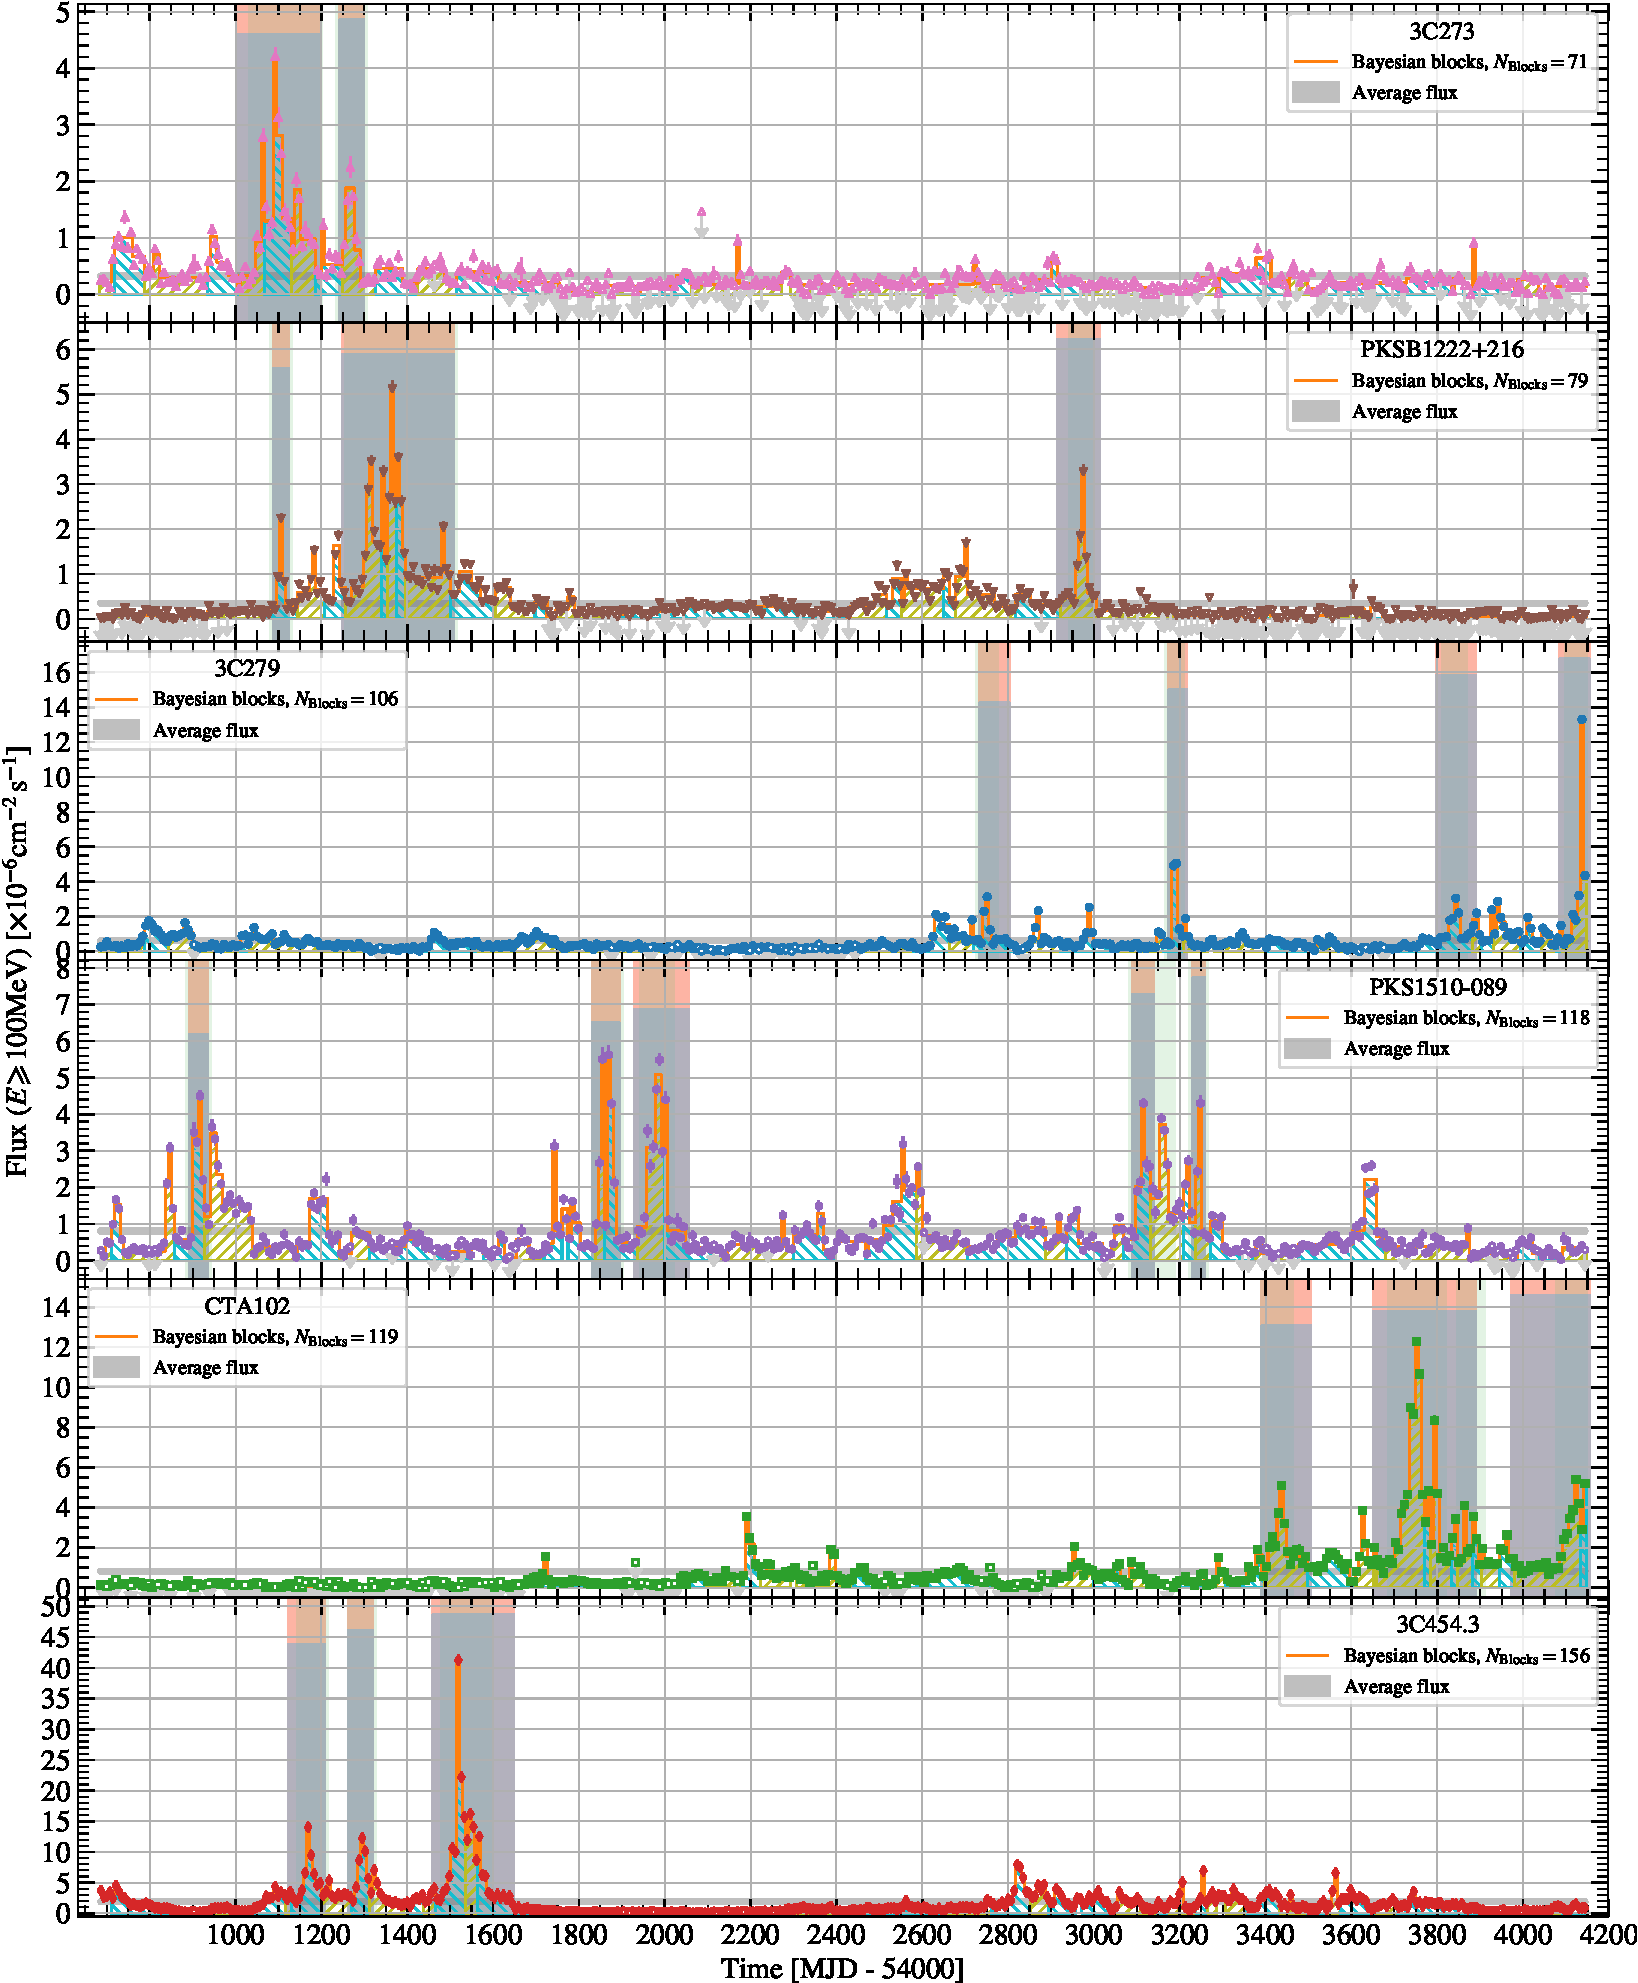
\includegraphics[width = .9\linewidth]{figures/lc_weekly_tsmin4.pdf}
    \caption{\gray light curves with weekly binning for the considered FSRQs. Open symbols denote upper limits at the $2\,\sigma$ confidence level.}
    \label{fig:weekly}
\end{figure*}

There is no generally accepted consensus to determine the data points that belong to a flaring state and which characterize the quiescent level. \citet{2013MNRAS.430.1324N} suggests a simple definition that a flare is a continuous time interval associated with a flux peak in which the flux is larger than half the peak flux value. 
This definition is intuitive, however, it is unclear how to treat overlapping flares and identify flux peaks in an unbiased way. To mitigate there problems, we have implemented one dimensional implementation of the HOP algorithm~\citep{Eisenstein:1997sm}.
The algorithm associates data points to their nearest neighbor weighted by flux.
We feed the BB representation of the light curve to the HOP algorithm and the resulting groups of data points are shown 
Fig.~\ref{fig:weekly} as left and right hatched areas. 
The combination of BBs and the HOP algorithm represents an unbiased way to split a light curve into quiescent and flaring episodes.

We iteratively zoom in on time ranges with bright \gray activity by identifying BBs with a flux, $F_{BB} \geqslant f_\mathrm{max}\overline{F}$ and including adjacent blocks with $F_{BB} \geqslant f_\mathrm{min}\overline{F}$. 
Overlapping time ranges are combined into one time range and the ranges are extended by one time bin on each side.
This method is preferred over using the HOP groups directly, since the HOP sheds might extend far from the peak flux of a flare. 
For the identified time span, we re-optimize the spectral model of the ROI in the same way as described in Sec.~\ref{sec:roi} but without re-localizing the central FSRQ or adding new point sources. Subsequently, we calculate a light curve with finer binning and again select the time ranges of the highest \gray activity. We repeat this procedure twice, down to a binning equal to the Good Time Intervals (GTI), of the \Fermi satellite which correspond to one passage of the source through the field of view of the satellite during one $\sim$ 95 minute orbit.
The choices of time binnings and values for $f_\mathrm{max}$ and $f_\mathrm{min}$ are summarized in Table~\ref{tab:zoom} together with the number of identified high \gray activity states (which might consists of several flares as indicated by the HOP groups).
The values of the threshold fluxes $f_\mathrm{max}, f_\mathrm{min}$ is somewhat arbitrary and are a compromise between including as many flares as possible but keeping the overall number of flares manageable. Note, that the sole purpose of this exercise is to select the brightest flares for  further analysis. 
The resulting time ranges for the weekly light curves are plotted as green shaded areas in Fig.~\ref{fig:weekly}.
The intermittent daily light curves are provided in Figs.~\ref{fig:daily-3c273-pks1222}-\ref{fig:daily-cta102-3c454} and  Figs.~\ref{fig:gti-3c273-pks1222}-\ref{fig:gti-cta102-3c454} show the GTI light curves. 
The source exposure can vary significantly between two adjacent orbits, as the satellite rocks between the celestial north and south pole in between orbits. This explains the large error bars on some of the time bins of the GTI light curves.

In a last step, we derive light curves on sub-GTI time scales. 
The time bin size is calculated from the adaptive binning method of \citet{lott2012}, where we choose bins of constant flux uncertainty of $\sim20\,\%$. 
In this step, we use the space craft information in time steps of 1\,s instead of 30\,s. Additionally, we compute the effective area in 5 bins of the azimuthal spacecraft coordinates since on such short time scales the exposure dependence on the azimuth cannot be averaged over.
\todo{show plots?}

\begin{deluxetable}{cccc}
\tablewidth{1\linewidth}
\tablecaption{ \label{tab:zoom} Thresholds for BB fluxes to select time ranges of \gray activity together with selected time binning and number of selected time ranges.
If no interval fulfills the $F_\mathrm{BB} \geqslant f_\mathrm{max}\overline{F}$ criterion but flux points exceed $5\times10^{-6}\,\mathrm{cm}^{-2}\,\mathrm{s}^{-1}$ we change $f_\mathrm{max}$ to 90\,\% the maximum value $F_\mathrm{BB}$.}
\tablehead{Binning & $f_\mathrm{min}$ & $f_\mathrm{max}$ & $N_\mathrm{time~ranges}$}
\startdata
7 days & 3 & 5 & 21\\
1 day & 2 & 3 & 31\\
GTI & 1 & 2 & 31\\
%Sub-GTI & -- & -- & --\\
\enddata
%\tablenotetext{a}{}
\end{deluxetable}

\todo{
\begin{enumerate}
\item move on to results
\item result section: divide into results of full time range with flux distribution, PSD, LCCF (I would leave that for the discussion part); GTI light curves with fitted light curve profiles and study of flare duration and symmetries -- energy dependent light curves? Or in discussion?; short time variability below orbital time scales; fits to the SEDs
    \item work extends previous works e.g. Naweljajko 2014 paper -- put in discussion?
    \item Describe data analysis
    \item finish table with sources listing Name, 3FGL name, RA, DEC, z, black hole mass, gravitational radius, Luminosity of Hbeta
\end{enumerate}
}
%%% Daily light curves %%%%%%%%%
\begin{figure*}
    \centering
    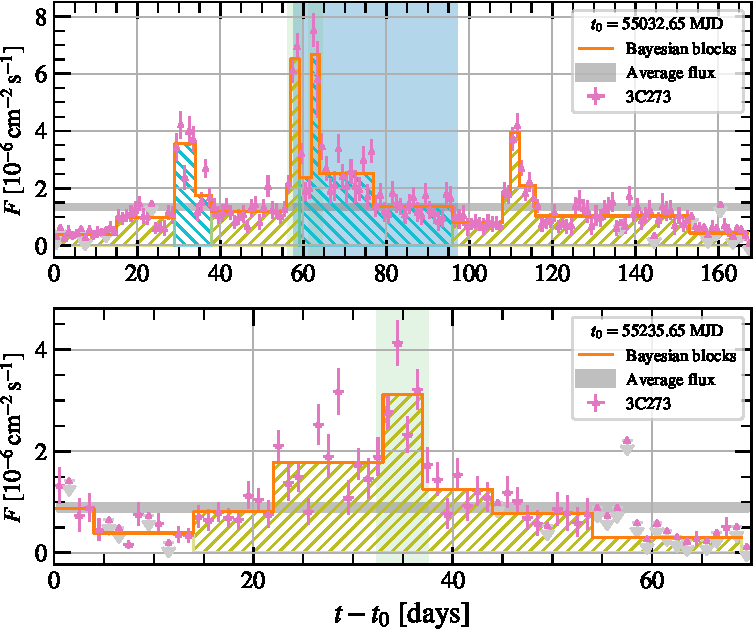
\includegraphics[width = .45\linewidth]{figures/lc_3C273_daily.pdf}
    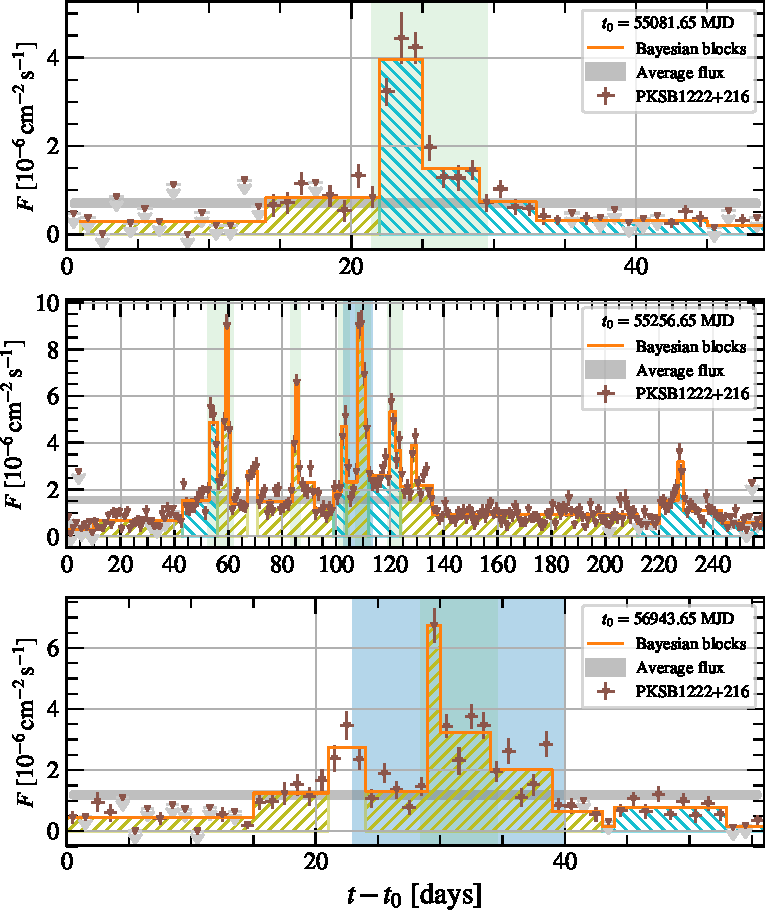
\includegraphics[width = .45\linewidth]{figures/lc_PKSB1222+216_daily.pdf}
    \caption{\label{fig:daily-3c273-pks1222}}
\end{figure*}

\begin{figure*}
    \centering
    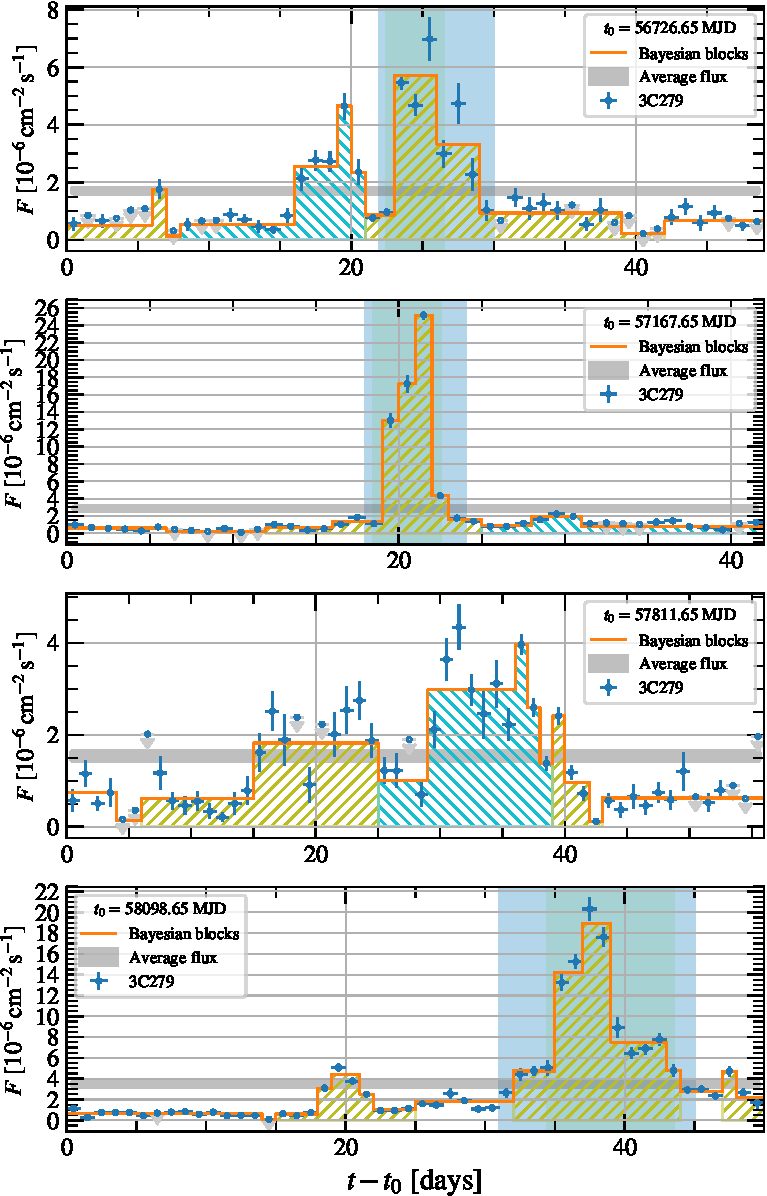
\includegraphics[width = .45\linewidth]{figures/lc_3C279_daily.pdf}
    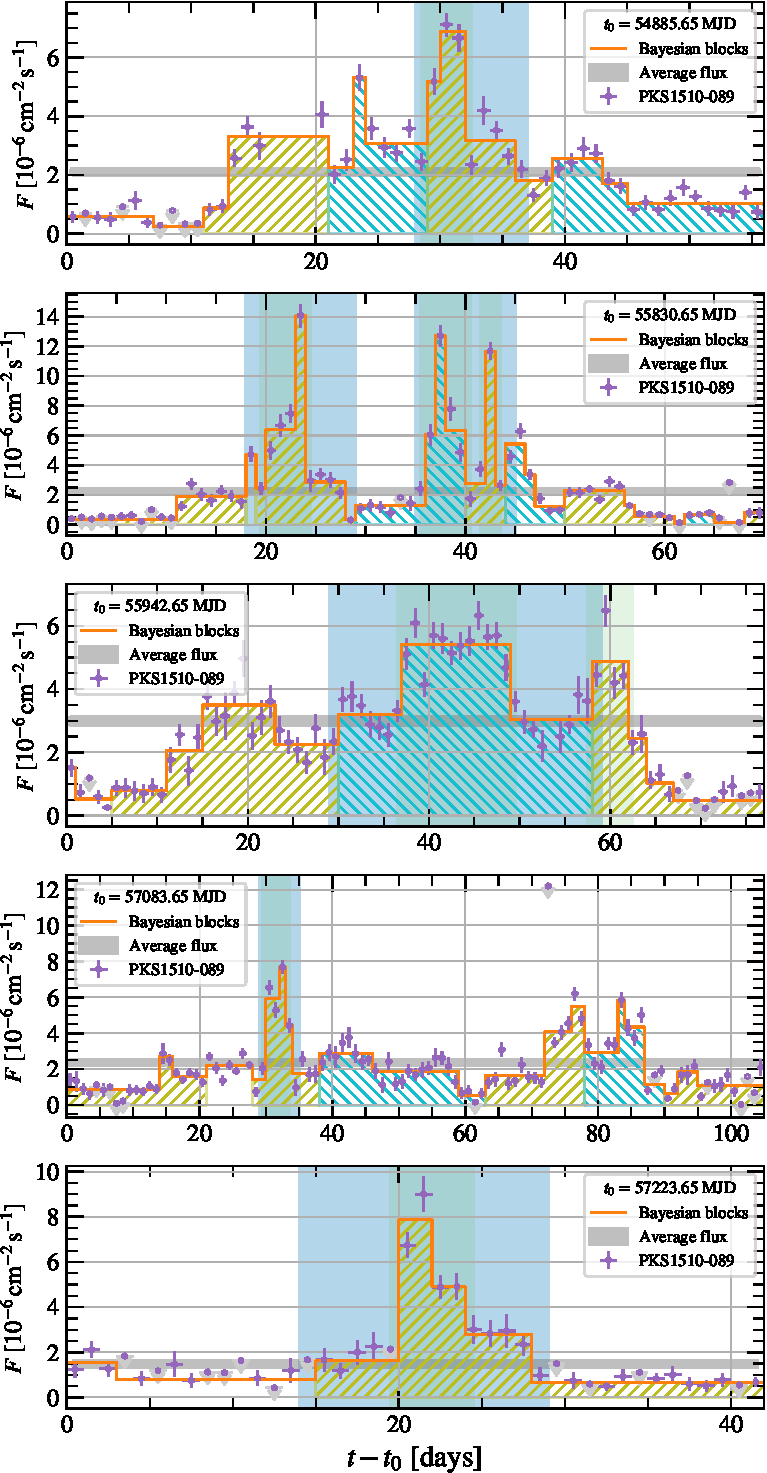
\includegraphics[width = .45\linewidth]{figures/lc_PKS1510-089_daily.pdf}
    \caption{\label{fig:daily-3c279-pks1510}}
\end{figure*}

\begin{figure*}
    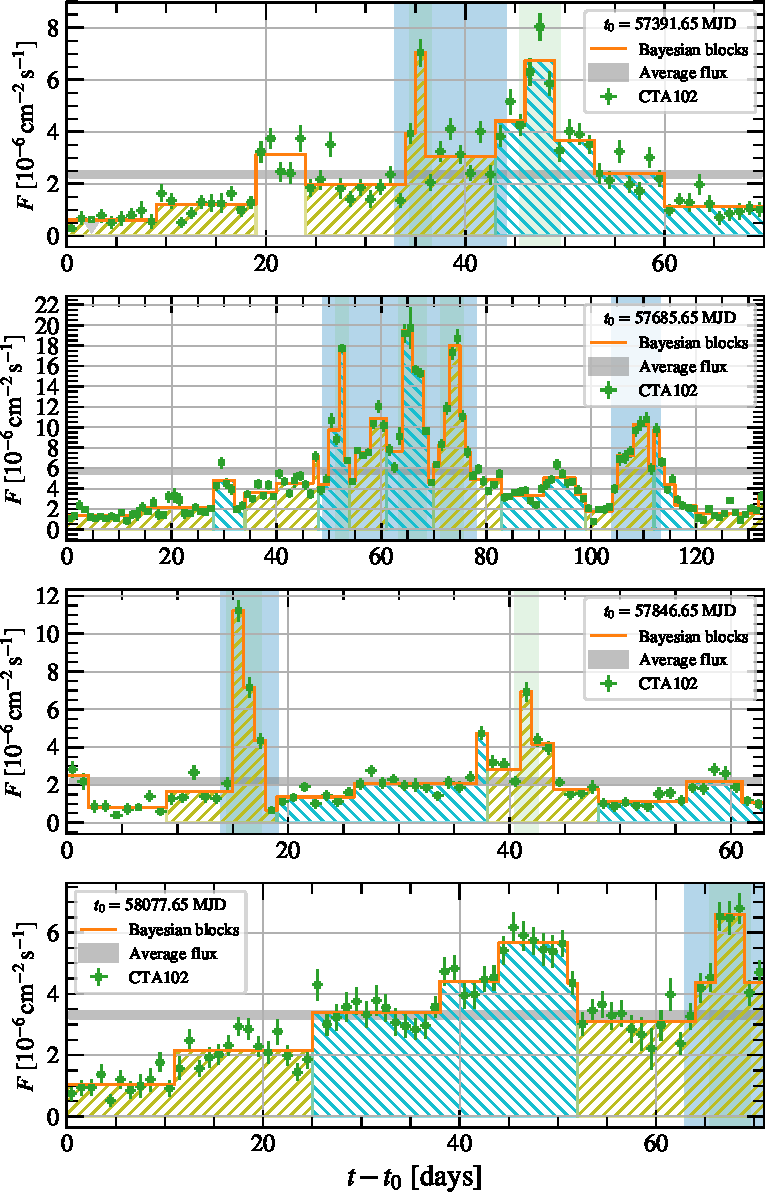
\includegraphics[width = .45\linewidth]{figures/lc_CTA102_daily.pdf}
    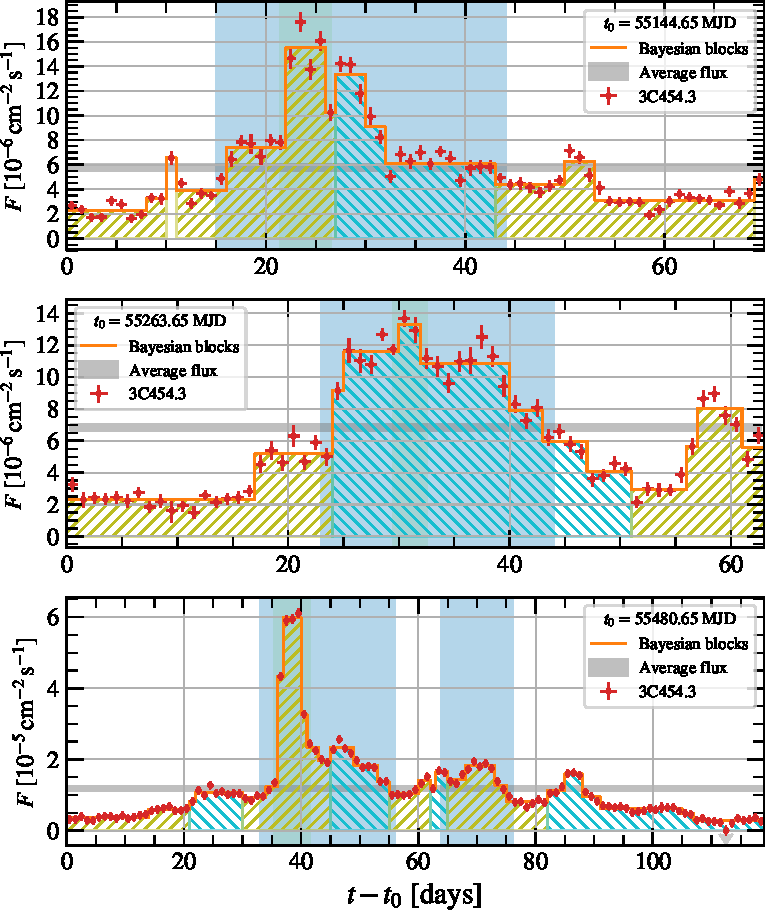
\includegraphics[width = .45\linewidth]{figures/lc_3C454p3_daily.pdf}
    \caption{\label{fig:daily-cta102-3c454}}
\end{figure*}
%%%%%%%%%%%%%%%%%%%%%%%%%%%%%%%%


%%% GTI light curves %%%%%%%%%
\begin{figure*}
    \centering
    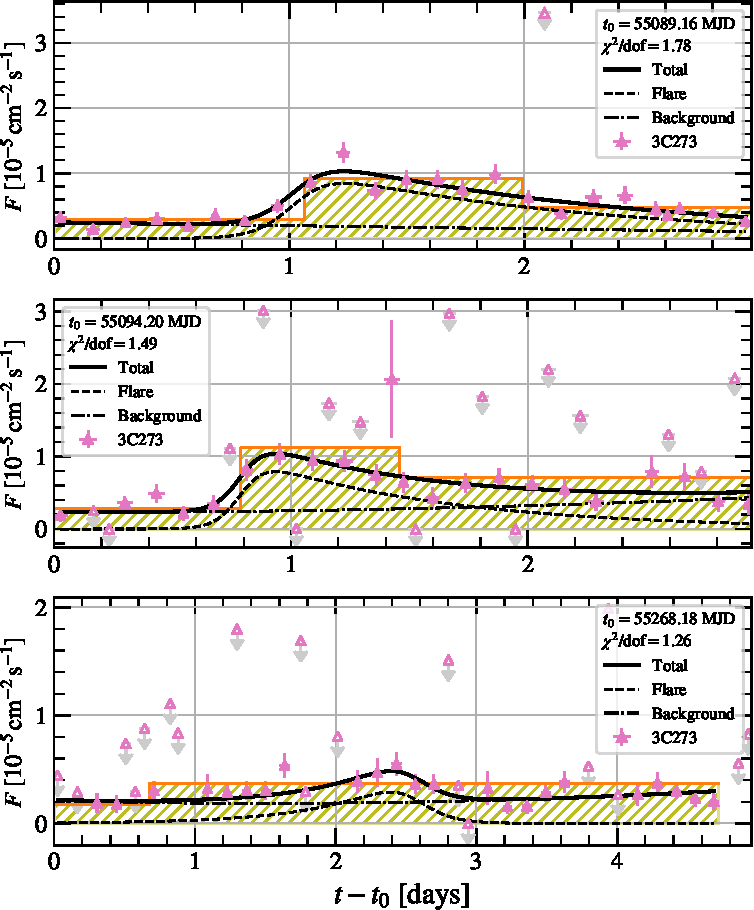
\includegraphics[width = .45\linewidth]{figures/lcfithop_3C273_orbit_all_maxiter2_fsys0p00_addcomp0_comb.pdf}
    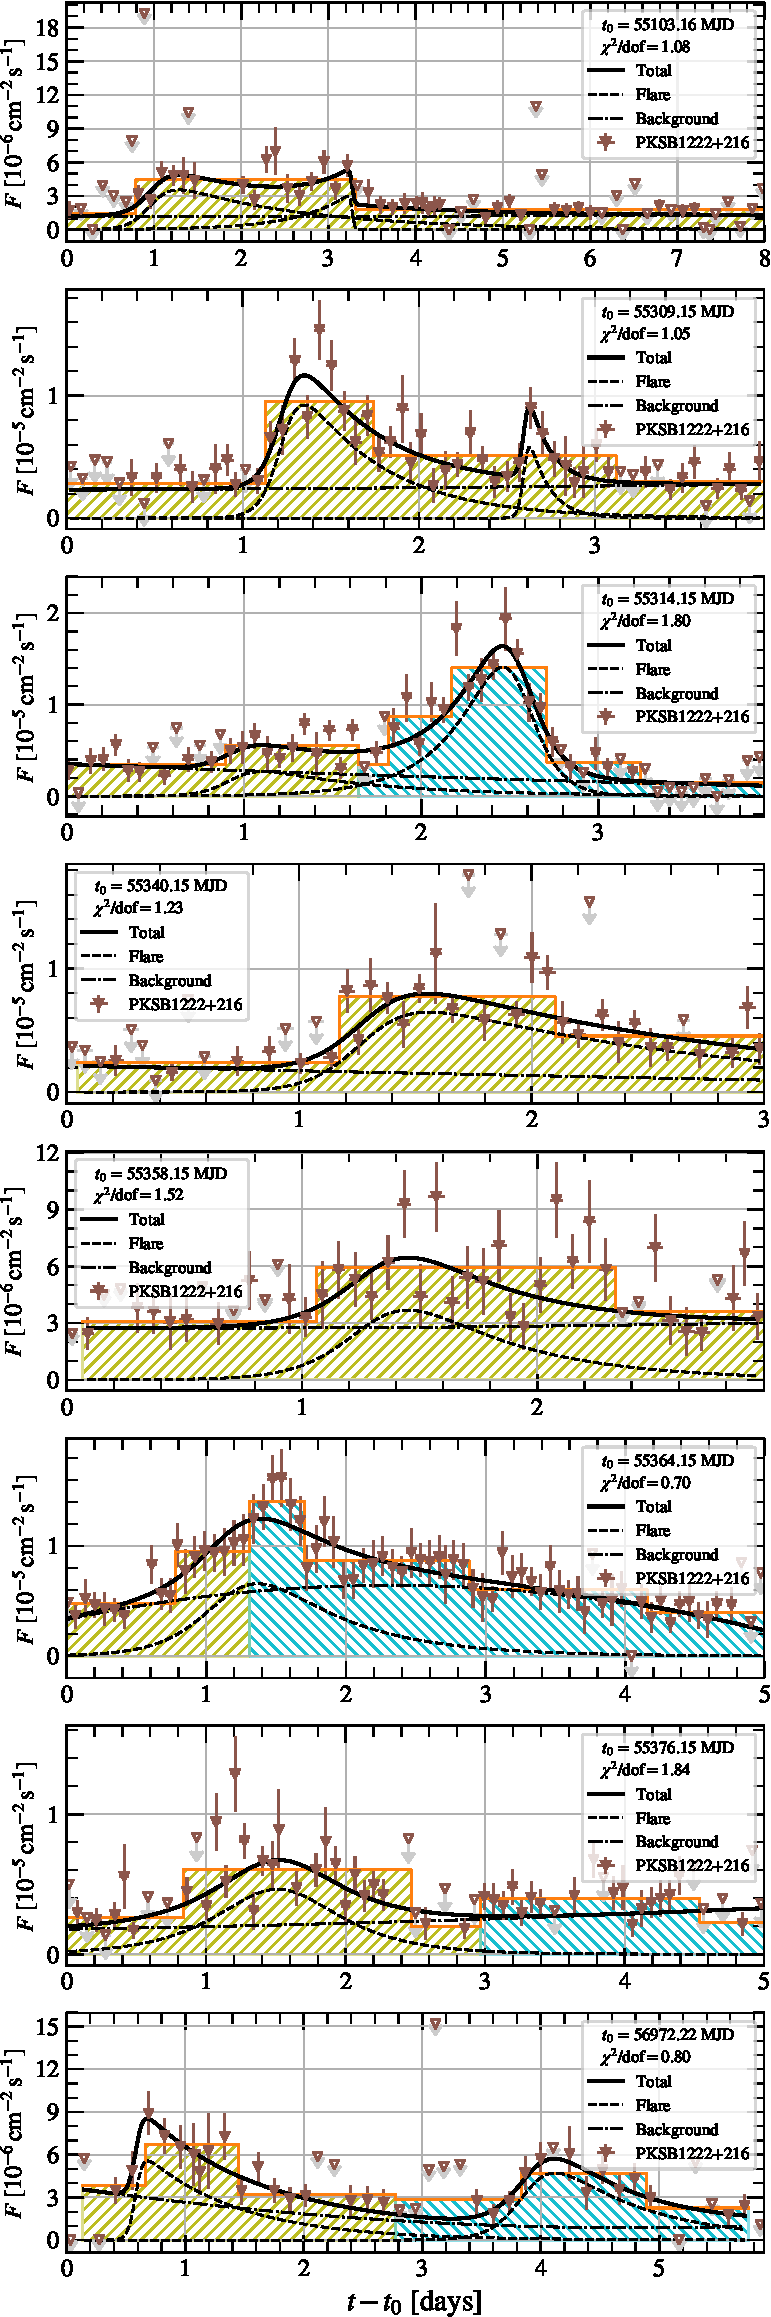
\includegraphics[width = .45\linewidth]{figures/lcfithop_PKSB1222+216_orbit_all_maxiter2_fsys0p00_addcomp0_comb.pdf}
    \caption{\label{fig:gti-3c273-pks1222}}
\end{figure*}

\begin{figure*}
    \centering
    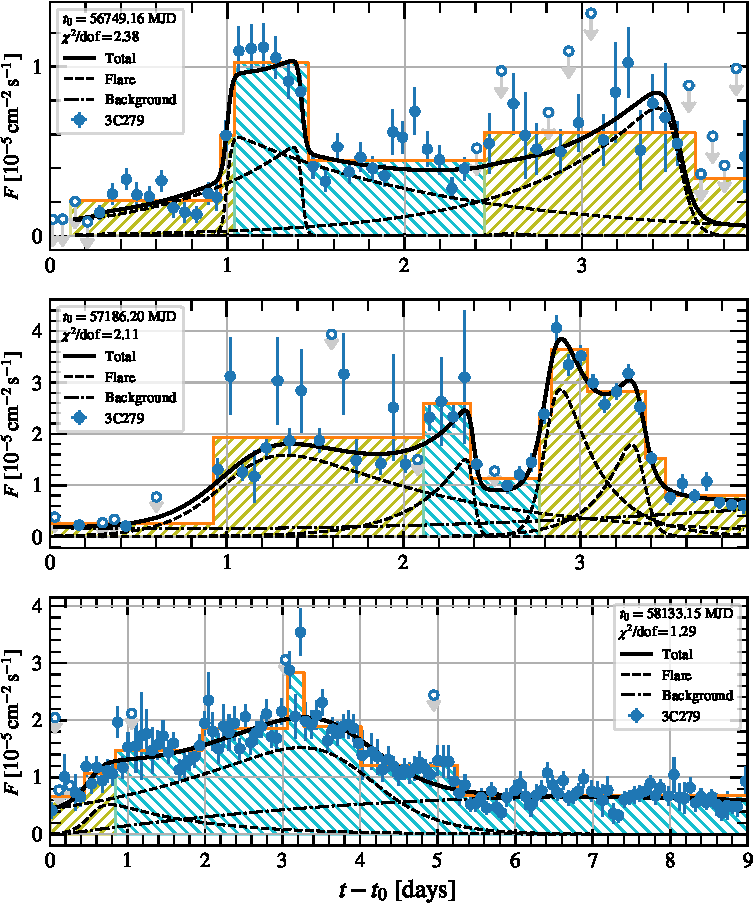
\includegraphics[width = .45\linewidth]{figures/lcfithop_3C279_orbit_all_maxiter2_fsys0p00_addcomp0_comb.pdf}
    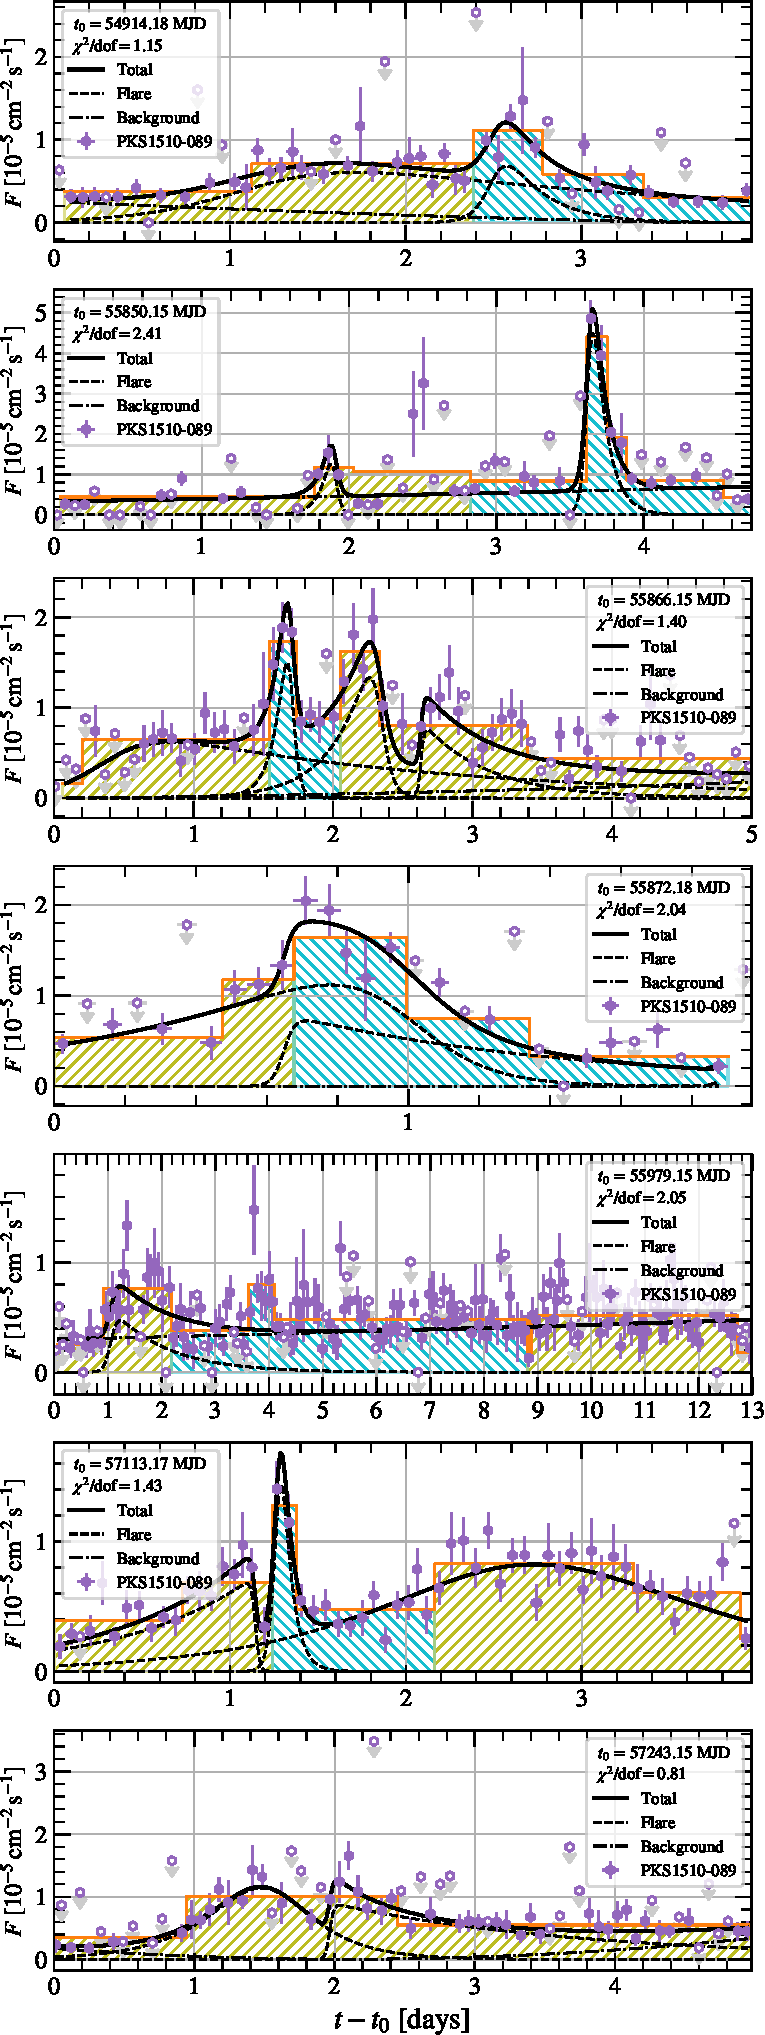
\includegraphics[width = .45\linewidth]{figures/lcfithop_PKS1510-089_orbit_all_maxiter2_fsys0p00_addcomp0_comb.pdf}
    \caption{\label{fig:gti-3c279-pks1510}}
\end{figure*}

\begin{figure*}
    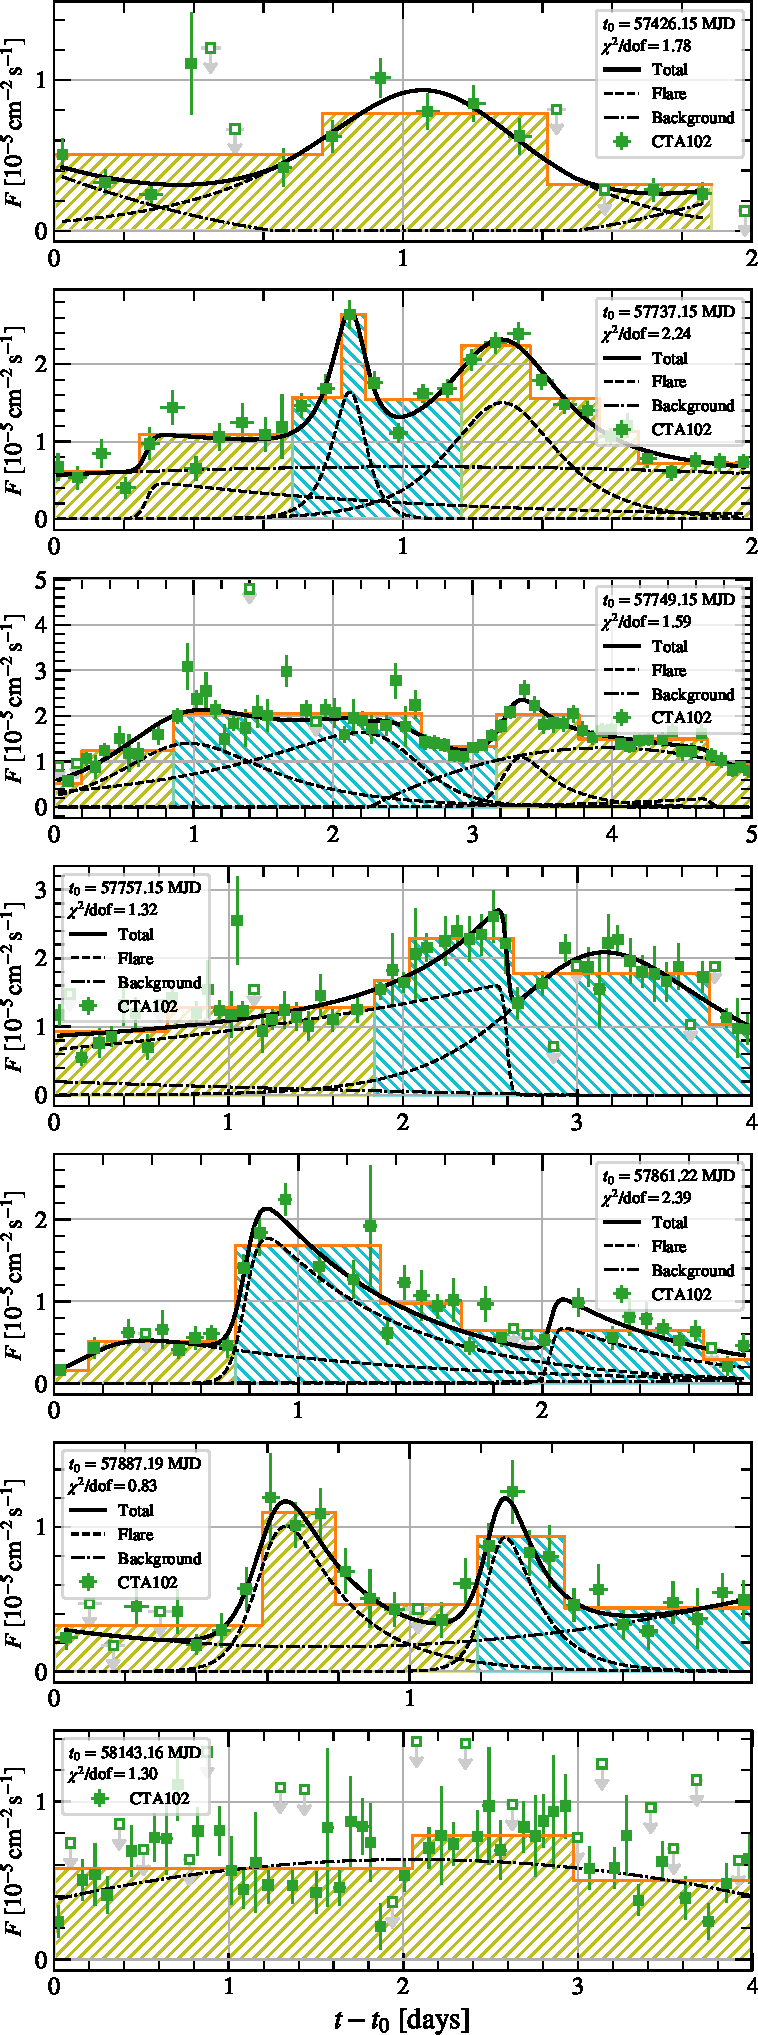
\includegraphics[width = .45\linewidth]{figures/lcfithop_CTA102_orbit_all_maxiter2_fsys0p00_addcomp0_comb.pdf}
    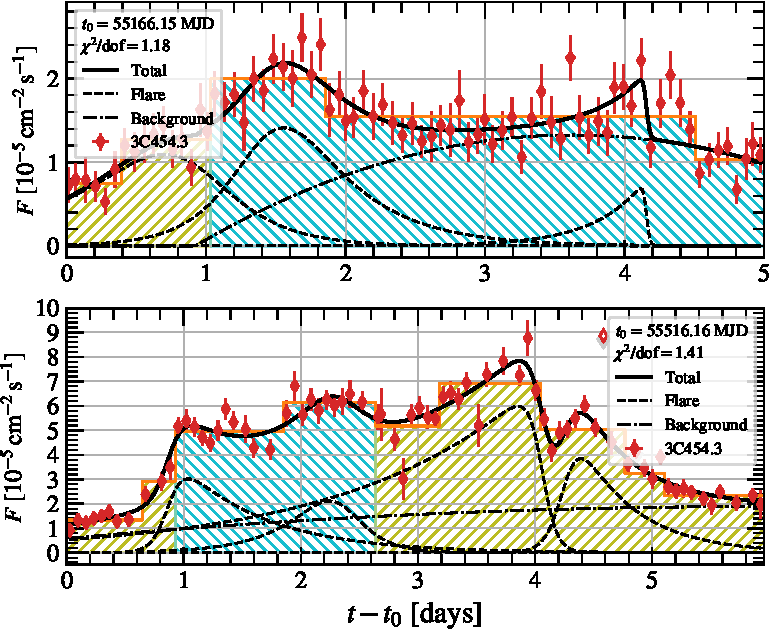
\includegraphics[width = .45\linewidth]{figures/lcfithop_3C454p3_orbit_all_maxiter2_fsys0p00_addcomp0_comb.pdf}
    \caption{\label{fig:gti-cta102-3c454}}
\end{figure*}
%%%%%%%%%%%%%%%%%%%%%%%%%%%%%%

\section{Results}
\label{sec:results}
We first present results derived from the weekly \gray light curves spanning the full 9.5\,year time range, which we refer to \emph{global light curve properties}, before deriving results from the local light curves on GTI and sub-GTI time scales.

\subsection{Global \gray light curves properties}
From the weekly light curves in Fig.~\ref{fig:weekly} it is qualitatively evident that the FSRQs show strong flares that exceed average flux by a factor of a few while the quiescent level is relatively stable. 
Such behavior is typical for FSRQs~\citet{}.
In order to quantify this behaviour we calculate probability distribution functions (PDF) of the fluxes by forming the histogram of the weekly fluxes per flux bin. 
The results are shown in Fig.~\ref{fig:fluxpdf}. The bins are chosen according to the algorithm of~\citet{knuth2006} and the error bars are calculated 


\begin{figure}
    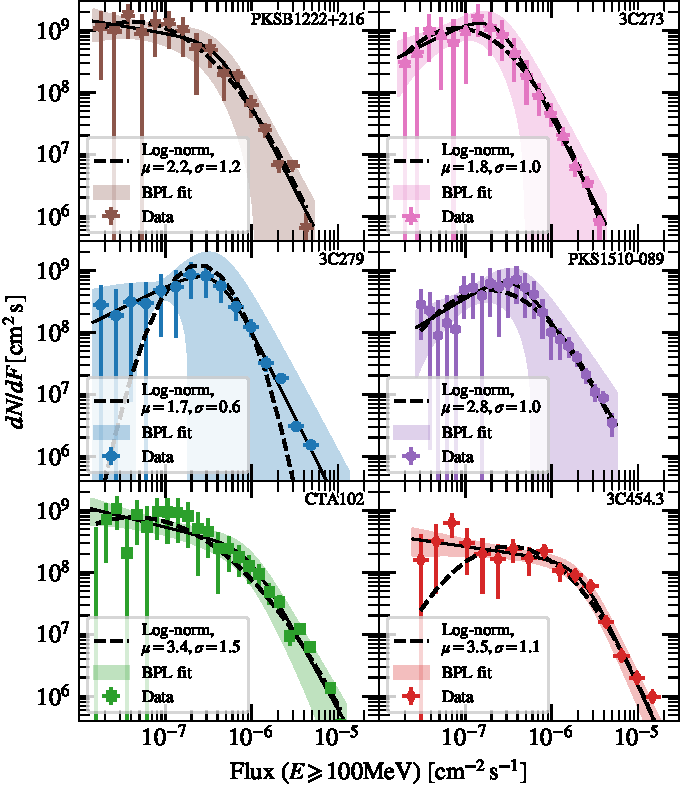
\includegraphics[width = .99\linewidth]{figures/fluxdist_weekly_tsmin9.pdf}
    \caption{\label{fig:fluxpdf}}
\end{figure}

\bibliography{mainbib}

%% This command is needed to show the entire author+affilation list when
%% the collaboration and author truncation commands are used.  It has to
%% go at the end of the manuscript.
%\allauthors

%% Include this line if you are using the \added, \replaced, \deleted
%% commands to see a summary list of all changes at the end of the article.
%\listofchanges


\end{document}

% End of file `sample62.tex'.
